\section{Deklaratives UI}
Im Gegensatz zu imperativen Frameworks wie dem \textit{Android SDK}
oder dem \textit{iOS UiKit} handelt es sich bei \textit{Flutter} um
ein so genanntes deklaratives Framework. Dies bedeutet,
dass das UI von Flutter immer den akutellen \textit{"State"} reflektiert.
Wird beispielsweise eine Option in den Einstellungen einer App geändert,
so ändert sich der \textit{"State"} der App welches das Neuzeichnen
der App auslöst (eine Checkbox wird gefüllt, ein Switch aktiviert).
Imperativ würde bedeuten, dass es Methoden wie \textit{widget.setText}
gibt um Werte direkt zu ändern. Hier wird der \textit{"State"} geändert
und das UI wird komplett neu gezeichnet.

\paragraph{Technisches Beispiel}\mbox{}
\hfill
\break

\begin{figure}[H]
    \centering
    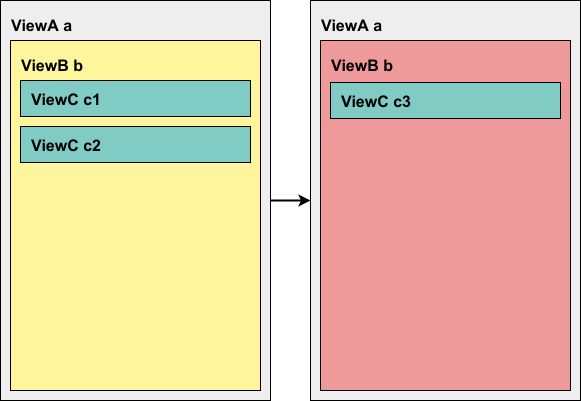
\includegraphics[width=0.8\columnwidth]{declarative_ui_example}
    \caption{Vergleich deklaratives \& imperatives UI}
\end{figure}
\newpage

Im imperativen Stil würde man eine Instanz \textit{b} des so
genannten \textit{Owners} der View \textit{ViewB} nutzen
und mit Hilfe eine Selektors wie beispielsweise \textit{findViewById}
Änderungen auf dieser anwenden (und somit diese implizit invalidieren).
Das kann ungefähr so aussehen:

\begin{figure}[H]
    \centering
    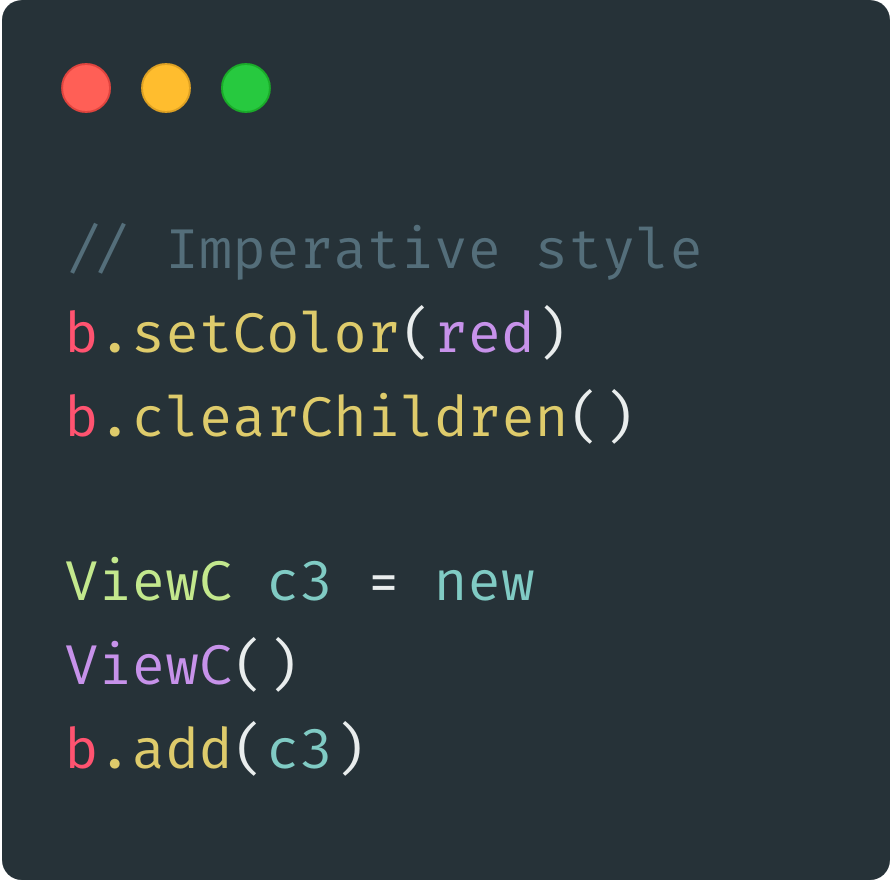
\includegraphics[width=0.4\columnwidth]{imperative_style}
    \caption{Beispiel: imperativer Stil}
\end{figure}

Außerdem müsste dieses Setup im Konstruktor von \textit{ViewB} dupliziert
werden, da die UI (der \ac{SPOT}) möglicherweise die Instanz \textit{b} überlebt.
Im deklarativen Frameworks sind View-Konfigurationen
(wie \textit{Flutter's} Widgets) unveränderlich (immutable) und an sich
nur simple Blaupausen. Um ein UI zu ändern, löst ein Widget einen Rebuild
auf sich selbst aus (in \textit{StatefulWidgets} häufig per \textit{setState()}
und erzeugt damit einen neuen Widget-Subtree.

\begin{figure}[H]
    \centering
    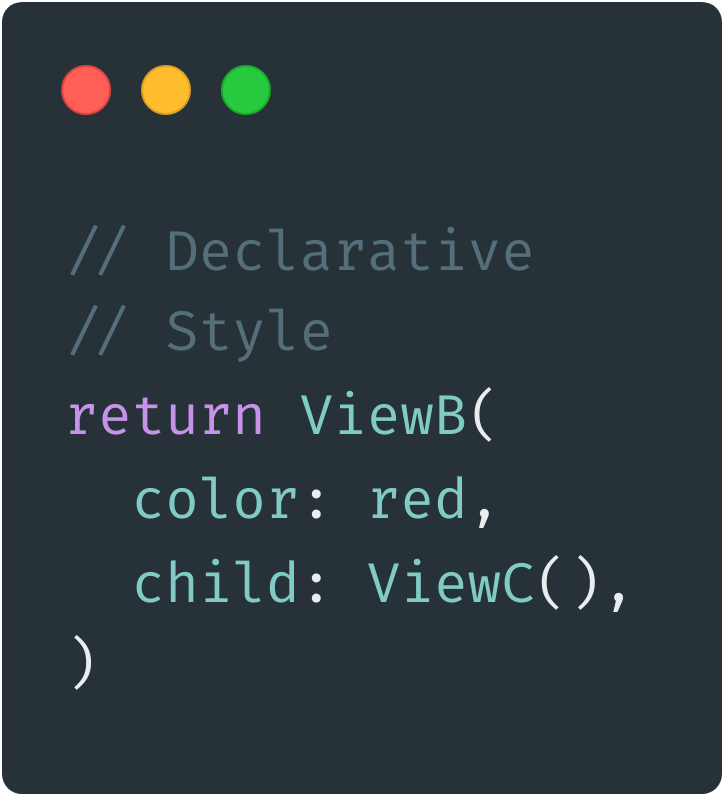
\includegraphics[width=0.4\columnwidth]{declarative_style}
    \caption{Beispiel: deklarativer Stil}
\end{figure}
